\documentclass{article}
\usepackage{graphicx}
\usepackage{minted}
\usepackage{parskip}
\usepackage[colorlinks,
            urlcolor=blue]{hyperref}
%\usepackage[margin=1in]{geometry}
\usepackage{amsmath}
\usepackage{amssymb}
\usepackage{fancyvrb}
\usepackage{booktabs}
\usepackage{url}
\usepackage{hyperref}
\usepackage{multirow}
\usepackage{pbox}
\usepackage[margin=1in]{geometry}

\author{Ashwin Srinath}
\title{An OpenCL-based tridiagonal solver for evaluation
    of compact finite differences on parallel architectures}
\begin{document}
% \renewcommand{\bibname}{References}

\section{Introduction}

    The motivation for this work comes from the need to evaluate
    \emph{compact finite differences} arising in large simulations of combustion.
    Compact finite different schemes result in
    high-order of accuracy for relatively small stencils.
    Numerical methods with small stencil widths are especially benefitial
    in managing communication costs in large-scale cluster computing.
    This work is concerned with implementing algorithms for evaluating
    compact finite differences to make full use of available parallel architecture.
    The target architecture studied is the NVIDIA Tesla K20 GPU.
    The algorithm design for this architecture is presented,
    along with the associated issues.
    Results are presented for domains sized up to $2048^3$ grid points,
    using up to 64 GPUs.

\section{Related work}



\section{Numerical method}

    We consider the following fourth-order
    compact finite difference scheme for evaluating the first derivative,
    with a 3-point stencil:

    \begin{equation}
        \alpha(f^{\prime}_{i-1} + f^{\prime}_{i+1}) + f^{\prime}_i
        =
        a\frac{f_{i+1} - f_{i-1}}{dx}
    \end{equation}

    For the particular scheme used, $\alpha = 1/4$,
    and $ a = 3/4 $.
    It is easily noted that this leads to a tridiagonal system of equations,
    along with a 3-point stencil to evaluate the RHS.
    Further, the left boundary can be treated using the following implicit equation:

    \begin{equation}
        f^{\prime}_1 + 2f^{\prime}_2 = \frac{-5f_1 + 4f_2 + f_3}{dx}
    \end{equation}

    The right boundary ($f^{\prime}_{n-1}$) is treated by utilizing
    the negative complex-conjugate of the Fourier image of the stencil
    at $f^{\prime}_1$:

    \begin{equation}
        f^{\prime}_{n-1} + 2f^{\prime}_{n-2}
        =
        \frac{5f_{n-1} - 4f_{n-2} - f_{n-3}}{dx}
    \end{equation}

    The tridiagonal system that needs to be solved for the derivatives,
    then has an LHS of the form:

    \[ %\arraycolsep=4pt
     \begin{bmatrix}
         1&2\\
         1/4&1&1/4\\
         &1/4&1&1/4\\
         &&1/4&1&1/4\\
         &&&1/4&1&1/4\\
         &&&&&\ddots\\
         &&&&&&\ddots\\
         &&&&&&&\ddots\\
         &&&&&&&2&1
      \end{bmatrix}
    \]

    And an RHS of the form:

    \[
     \begin{bmatrix}
         -5f_1 + 4f_2 + f_3\\
         f_{3} - f_{1}\\
         f_{4} - f_{2}\\
         \vdots\\
         \vdots\\
         \vdots\\
         \vdots\\
         f_{n} - f_{n-2}\\
         5f_{n} - 4f_{n-1} - f_{3}
      \end{bmatrix}
    \]

    A solution strategy is therefore concerned with the following:

    \begin{enumerate}
        \item{The evaluation of the right hand side.}
        \item{The solution of the resulting matrix system.}
    \end{enumerate}

\section{Reference approach}
    The current approach, developed for the CFDNS[ref] Compressible Navier-Stokes,
    and adapted to the Roadrunner[ref] architecture,
    is a parallel solver based on the standard LU algorithm,
    but specialized for the solution of a constant matrix.
    The problem is distributed among several ``processes'' and each
    process uses a single CPU core to perform computations.

    Assuming the coefficients of the LU algorithm are precomputed,
    the following steps are required to solve the tridiagonal system
    (only steps for the left-right sweep are listed, the right-left sweep
    consists of similar steps):

    \begin{enumerate}
    \item Precompute the arrays of coefficients of the LU algorithm---
    this is done once, in the beginning of the simulation process, and its cost
    can be neglected.
    \item Evaluate the RHS of the system.
    \item Compute $\hat{\phi_i}$ and $\hat{\psi_i}$ for each grid point $i$,
    with $\hat{\phi_i}$ and $\hat{\psi_i}$ both functions of the precomputed
    coefficient arrays and the right hand side.
    \item Every process posts the rightmost values of its $\hat{\phi_i}$ and $\hat{\psi_i}$,
        $\widetilde{\phi_k}$ and $\widetilde{\psi_k}$.
    \item Using the array of $\widetilde{\phi_k}$ and $\widetilde{\psi_k}$,
        each process computes $\widetilde{x_k}$, and uses it to compute
        $x_i,k = \phi_i + \psi_i\widetilde{x_k}$.
    \end{enumerate}

    The Message Passing Interface (MPI) is used for handling communication
    between processes.

\section{GPU architecture and parallelization strategies}

    The compact finite differences need to be evaluated
    at each grid point in the problem domain,
    shown in \ref{fig:domain}.
    Each grid point is represented as a cell in this representation.
    The domain has been shown as partitioned into blocks \ref{fig:one-block}.
    The blocks are three dimensional to facilitate
    the computation of derivatives in all three coordinate directions
    without incurring excessive communication costs.

    While evaluating the derivative, each block is assigned to a ``compute unit'',
    which may be a single core, a multi-core processor, or a GPU.
    Each block may be thought of as a collection of ``lines'' of grid points
    \ref{fig:one-line} in the x-direction,
    and the entire domain may be thought of as a collection of ``lines'' of
    blocks.
    While computing derivatives in other directions,
    (e.g., z-direction), we interpret each block as a collection of ``lines''
    of grid points in the z-direction and the domain as a collection of
    block in the z-direction.

    A GPU affords massive parallelism by virtue of several (thousand)
    lightweight compute threads (referred to as \emph{work items} in the OpenCL specification).
    The work items on a GPU are scheduled as \emph{blocks},
    which can be 1-D, 2-D, or 3-D.
    Each block is assigned to a \emph{streaming microprocessor}
    on the GPU---the Tesla K20 GPU has 13 streaming microprocessors---
    and runs in parallel.
    Threads within a block have common access to small, fast,
    \emph{shared memory}, which can be explicitly controlled.

    \subsection{Evaluation of the RHS}

        The RHS is evaluated by a 3 point stencil computation of
        the following form:

        \begin{equation*}
            r_i = \frac{3}{4dx} (f_{i+1} - f_{i-1})
        \end{equation*}

        This pointwise update can be performed easily in parallel
        for the internal points (points not close to the boundary of the process).
        Near the boundaries, the process will require information from its
        neighbours.

        Thus, each process will require information from its
        neighbouring processes every time the derivative needs to be evaluated.

        \begin{figure}[h]
        \begin{center}
        \includegraphics[trim={{100pt} {250pt} {100pt} {200pt}}, clip, height=200pt]{img/da-domain.eps}
        \end{center}
        \caption{Distribution of a 2-D domain among processes}
        \label{fig:da-domain}
        \end{figure}

        \begin{figure}[h]
        \begin{center}
        \includegraphics[trim={{100pt} {250pt} {100pt} {200pt}}, clip, height=200pt]{img/da-local-portion.eps}
        \end{center}
        \caption{Elements required by a process to evaluate RHS}
        \label{fig:da-local-portion}
        \end{figure}

        Thus, the RHS is evaluated in two steps:

        \begin{enumerate}
            \item Exchange boundary information with neighbouring processes
            \item Evaluate the RHS at each grid point (in parallel)
        \end{enumerate}

        The GPU is specialized for performing such a large number of independent
        computations as required in step 2.
        The RHS at each grid point is computing by a single work item
        (GPU thread).
        Therefore the number of work items scheduled is
        equal to the number of points in the local domain.

        Another popular strategy is to take advantage of
        shared memory, by launching 2-dimensional blocks of work-items,
        loading each into shared memory, and streaming the third dimension
        in registers.
        This approach is discussed in [ref], and is much more effective
        for larger stencils---as each thread in a block will access the same
        value several times, it is effective to use shared memory as explicitly
        controlled cache.

    \subsection{Solving the tridiagonal system}

        In the reference approach, a significantly larger portion of time is spent in solving
        the tridiagonal system in parallel.
        Because the problem does not exhibit the same degree of parallelism as
        the pointwise stencil update,
        the algorithms are necessarily more involved.

\section{Code design}

\section{Results and performance comparison}

    \subsection{Results for a single node}

    \begin{table}
    \centering
    \begin{tabular}{|l|r|r|r|r|}
    \hline
    Size    &      CPU (1 core) &  CPU (8 cores) & GPU (without memory transfers)  & GPU (with memory transfers) \\
    \hline
    32      &     0.0005        &   0.00029     &   0.00128 &   0.0014   \\
    64      &     0.0038        &   0.0008      &   0.0018  &   0.00385  \\
    128     &     0.042         &   0.0075      &   0.0073  &   0.02014  \\
    256     &     0.34          &   0.062       &   0.057   &   0.148    \\
    512     &     2.45          &   0.47        &   0.70    &   1.401    \\
    \hline
    \end{tabular}
    \caption{Performance of solvers on a single GPU (Tesla k20m)}
    \label{table:res1}
    \end{table}

    The results for a single node bring up some issues in performance evaluation.
    First, it is clear that the major cost for the GPU is not in the computational
    kernels, but rather in transferring data between host (CPU) and device (GPU) buffers.
    In the context of a larger piece of software,
    if only the computation of the compact finite difference was offloaded
    to the GPU, then considering this cost is absolutely essential.
    However, if the rest of the problem is also written to be solved on the GPU,
    then there is no need for transfers to and from the host at each
    time step.

    It is instructive also to examine the the total time


    We present the results for both

    \subsection{Results for multi-node}



    \subsection{Performance comparison}

    \subsection{Major concerns}

    \subsection{Performance improvement strategies}

\section{Computational practices}

% left, lower, right, upper
\begin{figure}[h]
\begin{center}
\includegraphics[trim={{100pt} {150pt} {100pt} {150pt}}, clip, height=250pt]{img/domain.eps}
\end{center}
\caption{Domain}
\label{fig:domain}
\end{figure}

\begin{figure}[ht]
\begin{minipage}[b]{0.45\linewidth}
\centering
\includegraphics[trim={{50pt} {150pt} {50pt} {150pt}}, clip, height=200pt]{img/one-block.eps}
\caption{Single block}
\label{fig:one-block}
\end{minipage}
\hspace{0.5cm}
\begin{minipage}[b]{0.45\linewidth}
\centering
\includegraphics[trim={{50pt} {150pt} {50pt} {150pt}}, clip, height=200pt]{img/one-thread.eps}
\caption{Single thread}
\label{fig:one-line}
\end{minipage}
\end{figure}




\begin{figure}[h]
\begin{center}
\includegraphics[trim={{100pt} {150pt} {100pt} {150pt}}, clip, height=300pt]{img/parallel-x.eps}
\end{center}
\caption{Parallel x}
\label{fig:parallel-x}
\end{figure}




\begin{figure}[h]
\begin{center}
\includegraphics[trim={{100pt} {150pt} {100pt} {150pt}}, clip, height=300pt]{img/parallel-yz.eps}
\end{center}
\caption{Parallel yz}
\label{fig:parallel-yz}
\end{figure}




\begin{figure}[h]
\begin{center}
\includegraphics[trim={{100pt} {150pt} {100pt} {150pt}}, clip, height=300pt]{img/parallel-both.eps}
\end{center}
\caption{Parallel-both}
\label{fig:parallel-both}
\end{figure}



\end{document}
